\documentclass[10pt]{article}
\usepackage[letterpaper,left=0.48in,right=0.48in,top=0.40in,bottom=0.38in]{geometry}
\usepackage[T1]{fontenc}
\usepackage{lmodern}
\usepackage{amsmath,amssymb,mathtools}
\usepackage{graphicx}
\usepackage{array,tabularx}
\usepackage{microtype}
\usepackage{hyperref}
\usepackage{embedfile}
\hypersetup{hidelinks}
\pagestyle{empty}
\setlength{\parindent}{0pt}
\setlength{\parskip}{0pt}
\setlength{\tabcolsep}{3pt}
\renewcommand{\arraystretch}{1.34}
\setlength{\extrarowheight}{2.2pt}
\newcolumntype{L}{>{\raggedright\arraybackslash\bfseries}p{1.23in}}
\newcolumntype{M}{>{\raggedright\arraybackslash}X}
\newcommand{\C}{\mathbb C}
\newcommand{\Z}{\mathbb Z}
\newcommand{\Fh}[4]{{}_2F_1\!\left(#1,#2;#3;#4\right)}
\begin{document}

{\Large\bfseries Trefoil Symplectic-Period Certificate}\hfill
{\small Bradley Klee, Mech.An.ika Sol (OpenAI)}

\vspace{4pt}\hrule\vspace{7pt}

\begin{center}
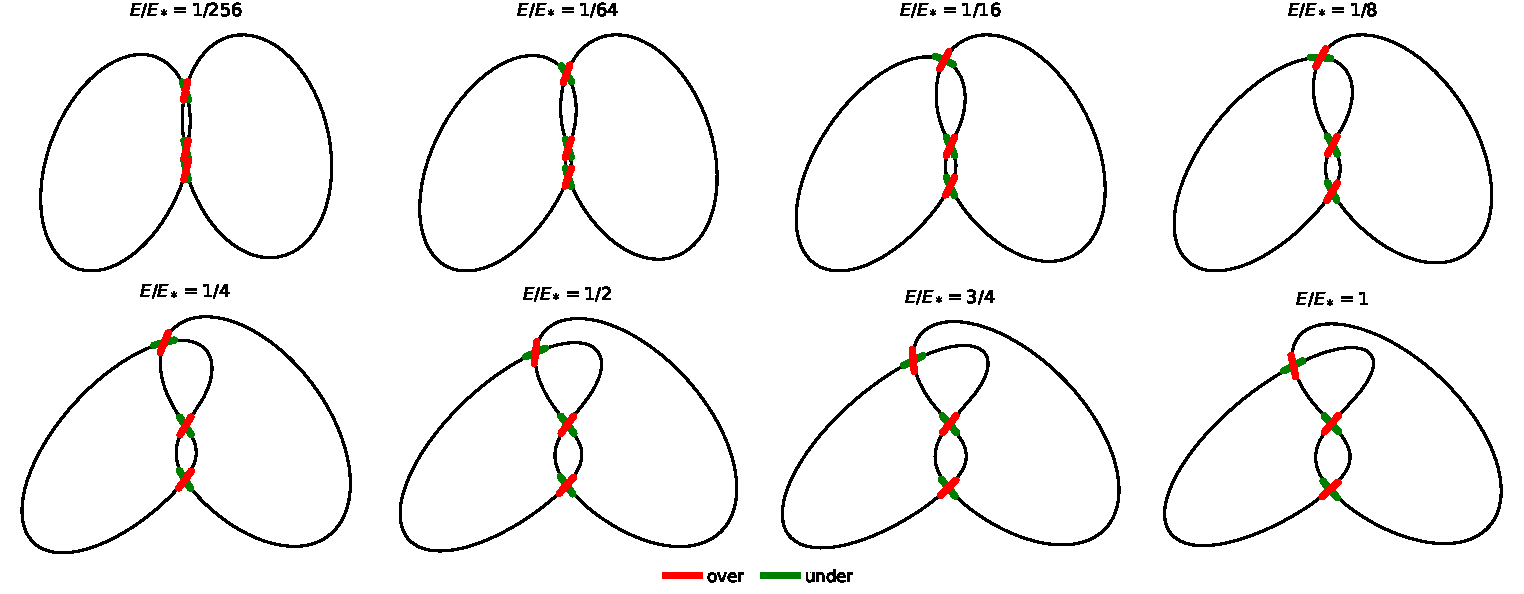
\includegraphics[width=0.98\textwidth,height=2.42in,keepaspectratio]{trefoil_energy_family_view2.pdf}
\end{center}
\vspace{-3pt}
{\footnotesize
\textbf{Computed family.}
Complete stereographic images of $K_E$, shape-normalized by $R=\sqrt E$, with one fixed screen view. Short green/under and red/over segments are centered at the computed crossings and red is always drawn last. The range ends at the first positive ODE singularity $E_*=4/27$, not at a knot transition.}

\vspace{6pt}\hrule\vspace{5pt}

\small
\begin{tabularx}{\textwidth}{L M}
Model &
$C=\{z^2=w^3\}\subset(\C^2,\omega_0)$, \quad
$\omega_0=\frac{i}{2}(dz\wedge d\bar z+dw\wedge d\bar w)$, \quad
$H=|z|^2+|w|^2$, \quad $K_E=C\cap H^{-1}(E)$.\\
Parametrization &
$z=s^3=u^{3/2}e^{3i\theta}$, \quad $w=s^2=ue^{2i\theta}$, \quad
$E=h(u)=u^3+u^2=u^2(u+1)$, \quad $u>0$.\\
Restricted forms &
$\lambda_0=\frac12\operatorname{Im}(\bar z\,dz+\bar w\,dw)$, \quad
$\lambda_C=\frac12(3u^3+2u^2)d\theta$, \quad
$\omega_C=d\lambda_C=\frac12(9u^2+4u)du\wedge d\theta$.\\[2.5pt]
Time form &
$dh=(3u^2+2u)du$, \quad $\omega_C=dh\wedge\eta$, \qquad
$\displaystyle \eta=\frac{9u+4}{2(3u+2)}d\theta$, \quad
$\iota_{X_h}\omega_C=-dh$, $\eta(X_h)=1$.\\[5pt]
Period / action &
$\displaystyle T(E)=\oint_{K_E}\eta=\pi\frac{9u+4}{3u+2}$, \qquad
$\displaystyle A(E)=\oint_{K_E}\lambda_C=\pi(3u^3+2u^2)$, \qquad
$\displaystyle \frac{dA}{dE}=T(E)$.\\[5pt]
\end{tabularx}

\vspace{4pt}\hrule\vspace{5pt}

\begin{tabularx}{\textwidth}{L M}
Energy-native function &
$\displaystyle \Phi(E)=3-\frac{T(E)}{\pi}=\frac{2}{3u+2}$, \qquad
$\displaystyle u=\frac{2(1-\Phi)}{3\Phi}$.\\[4pt]
Algebraic elimination &
Substituting $E=u^2(u+1)$ gives
$\displaystyle (4-27E)\Phi^3-12\Phi+8=0$.\\[3pt]
Direct derivatives &
$\displaystyle \Phi_E=-\frac{6}{u(3u+2)^3}$, \qquad
$\displaystyle \Phi_{EE}=\frac{12(6u+1)}{u^3(3u+2)^5}$.\\[4pt]
ODE &
$\displaystyle E(27E-4)\Phi''+2(27E-1)\Phi'+6\Phi=0$.\\[3pt]
Gauss form &
With $\displaystyle x=\frac{27E}{4}$ and $\Phi(E)=y(x)$,
$\displaystyle x(1-x)y''+\left(\frac12-2x\right)y'-\frac29y=0$.\\[4pt]
Solution &
$\displaystyle \Phi(E)=
\Fh{\frac13}{\frac23}{\frac12}{\frac{27E}{4}}
-\frac32\sqrt E\,
\Fh{\frac56}{\frac76}{\frac32}{\frac{27E}{4}}$.\\[5pt]
Branch sign &
For $E>0$, $u>0$ and hence $\Phi(E)=2/(3u+2)<1$; therefore
$\displaystyle \Phi(E)=1-\frac32\sqrt E+O(E)$ and the minus sign is forced.\\
\end{tabularx}

\vspace{4pt}\hrule\vspace{5pt}

\begin{tabularx}{\textwidth}{L M}
Integral uniformizer &
Only now set $\displaystyle q=\frac{\sqrt E}{4}$ and $G(q)=\Phi(16q^2)$. Then\\[-1pt]
& $\displaystyle G(q)=1-6q+48q^2-420q^3+3840q^4-36036q^5+344064q^6-3325608q^7+\cdots$.\\[4pt]
Coefficients &
$\displaystyle G(q)=\sum_{n\ge0}(-1)^na_nq^n$, \qquad
$\displaystyle a_n=4^n\binom{3n/2}{n}\in\Z$, \qquad
$\displaystyle a_n=[x^n]\big((1-x)(1-2x)\big)^{-n-1}$.\\[5pt]
Recurrence / OEIS &
$\displaystyle (n+1)(n+2)a_{n+2}=12(3n+4)(3n+2)a_n$, \quad
$a_0=1$, $a_1=6$. \quad Unsigned coefficients: \textbf{OEIS A244038}.\\[2pt]
First terms &
$1,\ 6,\ 48,\ 420,\ 3840,\ 36036,\ 344064,\ 3325608,\ 32440320,\ 318704100,\ldots$\\
Numerical audit &
On the original $K_E\subset\mathbb R^4$ at eight energies $10^{-4}\le E\le1$ (including $4/27$): constrained-flow quadrature agrees with $T(E)$ to $8.3\times10^{-11}$ relative; an independent polygonal $\oint\lambda_0$ plus centered $E$-difference gives $1.4\times10^{-8}$.\\
\end{tabularx}

\vspace{4pt}\hrule\vspace{4pt}

\footnotesize
\textbf{Embedded verification payload.}
Attachments include JSON data, exact SymPy and numerical verifiers, crossing audit, figure code, and this source. They check the forms, cubic/ODE/Gauss pullback, branch sign, integer series/recurrence, numerical integrals, and all eight three-crossing projections. SHA-256: \texttt{a25dcacbb8100a31\ldots d4ea6b1afa5e23}.

\embedfile[desc={Trefoil exact verification payload}]{trefoil_period_payload.json}
\embedfile[desc={Trefoil exact SymPy verifier}]{verify_trefoil.py}
\embedfile[desc={Trefoil independent numerical audit}]{numerical_audit.py}
\embedfile[desc={Trefoil numerical audit output}]{numerical_audit.json}
\embedfile[desc={Trefoil crossing audit data}]{crossing_family_view2.json}
\embedfile[desc={Trefoil figure generator}]{make_figures.py}
\embedfile[desc={Trefoil certificate LaTeX source}]{trefoil_certificate_v4.tex}

\end{document}
